\section{Minimal Axioms of Intelligence}


\subsection{Overview}


\S{}2 では、知性を「停止構造を生み出し続けながら、自身は停止しない持続運動」として位置づけ、知覚・認識・知識・知性の四層分離を行った。本セクションでは、この層分離を構造的に支える条件 ── すなわち知性層に対応する持続運動が成立するための \textbf{最小公理} ── を提示する。

ここでの目的は知性の定義ではなく、\textbf{下限の定式化} である。本セクションが提示する三公理を満たさない動的系は、\S{}2 で述べた意味での知性的動態を持続させにくい。逆に、これら三公理を同時に満たす動的系は ── substrate やスケールに関わらず ── \S{}2 が述べた持続運動の最小構造を備えうる。

本セクションの公理は \textbf{意図的に最小} である。意味・目的・判断・正しさ・主体性 ── これらの規範的または意味論的概念は、公理レベルでは一切導入されない。これらは上位層あるいは解釈投影として後から現れうるが、知性の構造的成立には不要である。この \textbf{意味論的中立性} が、本論文が領域横断的(\S{}5)かつ哲学的応用可能(\S{}6)である根拠となる。

\subsection{Axiom I: Connected state space}


第一の公理は、\textbf{連結された状態空間} の存在である。

形式的に、可能な状態の集合を

\[
\mathcal{S} = \{ s_1, s_2, \dots \}
\]

と書く。連結性の要請は、状態が孤立せず、状態間に \textbf{直接または間接の関係} ── 遷移、影響、依存 ── が存在することを意味する。

連結性の重要な特徴は、それが \textbf{連続的位相を要求しない} という点である。離散グラフ構造で十分である ── ただし、ある状態から他の状態への到達が、何らかの遷移列を通じて可能でなければならない。状態の単なる列挙(関係構造なき集合)は、本公理の意味での連結状態空間ではない。

連結性が満たされない場合に何が失われるかを示す:

\begin{itemize}
\item 状態間に到達可能性がなければ、情報は伝播も累積もしない
\item 系は孤立した反応の集合に縮退し、過去の状態が現在に影響しない
\item 学習・適応・統合のいかなる構造も成立しない
\end{itemize}

つまり連結性は、\textbf{動的系が単一の系として振る舞うため} の最小条件である。連結性なき系は、形式的には複数系の集合であり、知性的動態の主体となりえない。

\subsection{Axiom II: Temporal ordering}


第二の公理は、\textbf{時間的順序付け} である。状態更新は順序を持って起こらねばならず、先行する状態が後続の状態を制約しなければならない。

抽象的には:

\[
s(t+1) = F(s(t))
\]

ただし写像 $F$ の具体形は本公理では指定されない。

\textbf{重要な注意点が三つある。}

第一に、時間的順序付けは \textbf{外部時計を要求しない}。物理的な絶対時間の存在は不要であり、必要なのは「更新が同時には起こらない」「変化が瞬時に消失せず累積する」という構造的順序のみである。これは VED で言う差分発展構造と整合的である \citep{VEDVol1}。

第二に、時間的順序付けは \textbf{方向性} を含意する。$s(t+1) = F(s(t))$ という記述は、過去から未来への一方向性を持つ。可逆系であっても、状態変化の \textbf{記録性} ── すなわち過去の影響が現在に痕跡を残すこと ── が要請される。

第三に、時間的順序付けは \textbf{離散か連続かを問わない}。離散時間ステップでも連続力学系でも、上記の構造的条件が満たされれば公理を充足する。

時間順序が失われる場合の退化様式:

\begin{itemize}
\item 同時更新が支配的になれば、状態は瞬時平均化し、構造形成が起こらない
\item 変化が累積されなければ、履歴依存的構造(学習、適応、理解と関連する一切)が形成不可能になる
\item 時間的方向性なき系は、本質的に静的な系であり、いかなる動態も持たない
\end{itemize}

時間順序は、\textbf{動的系が履歴を持つため} の最小条件である。

\subsection{Axiom III: Global constraint $\Phi$}


第三の公理は、\textbf{グローバル制約} $\Phi$ の存在である。$\Phi$ は系全体の動態にバイアスを与え、これを安定化させる。

形式的に、$\Phi$ は状態空間上のスカラー場として表現される:

\[
\Phi : \mathcal{S} \rightarrow \mathbb{R}.
\]

$\Phi$ の構造的役割を理解するには、まず \textbf{何を $\Phi$ ではない} かを明示することが重要である。

\textbf{$\Phi$ は目的でも意味でも価値でもない。} これらの規範的概念は、本公理のレベルでは導入されない。$\Phi$ は構造的バイアスとしてのみ機能し、状態遷移を方向づけ、無制御の発散を防ぐ。

\textbf{$\Phi$ は局所更新規則の単純集約に還元されない。} これが本公理の最も重要な特徴である。すべての局所遷移が well-defined であっても、グローバル制約が欠如すれば動態は拡散・不安定化・断片化する。逆に、$\Phi$ の存在は局所規則からは導出できない大域的整合性を生む。

この \textbf{非還元性} は、$\Phi$ の現れ方の多様性を許す:

\begin{itemize}
\item 物理系では、$\Phi$ はポテンシャル場、ハミルトニアン、エントロピー関数として現れる
\item 生命系では、$\Phi$ は栄養勾配、境界条件、代謝制約として現れる
\item 人工系では、$\Phi$ は損失関数、報酬構造、訓練分布として現れる
\end{itemize}

これらは表現上は異なるが、構造的役割は同じである ── すなわち局所更新規則を超えて、系全体の動態を方向づける大域的バイアスである。

$\Phi$ が欠如する場合の退化様式:

\begin{itemize}
\item 局所更新は well-defined でも、全体の動態は無方向の拡散に帰着する
\item 系は最終的に最大エントロピー状態へと向かい、構造形成を持続できない
\item 局所最適化のみが起こり、大域的整合性は喪失する
\end{itemize}

$\Phi$ は、\textbf{動的系が単一の方向性を持つため} の最小条件である。

\subsection{The joint necessity of the three axioms}


三公理のいずれも、それ単独では不十分である。本小節では、各公理を一つずつ欠いた場合の退化様式を構造的に整理する。

\textbf{公理 I のみを欠く場合}(時間順序 + $\Phi$ だが連結性なし):
系は局所最適化のみを行う。各孤立部分は内部で動態を持ちうるが、系全体としての統合は起こらない。これは「複数の独立した動的系の集合」であって、単一の知性的動態ではない。

\textbf{公理 II のみを欠く場合}(連結性 + $\Phi$ だが時間順序なし):
系は静的固定に向かう。連結された状態空間と大域的バイアスがあっても、状態変化が累積されなければ系は瞬時に均衡状態へと収束し、その後動かない。これは「凍結した最適化問題の解」であって、持続する動態ではない。

\textbf{公理 III のみを欠く場合}(連結性 + 時間順序だが $\Phi$ なし):
系は反応系または記録系に退化する。状態遷移は起こり、履歴も形成されるが、大域的方向性が欠如するため、系全体としては無方向の拡散に向かう。これは「履歴を持つランダム過程」であって、構造的整合性を持つ動態ではない。

\begin{table}[H]
\centering
\small
\begin{tabularx}{\textwidth}{>{\raggedright\arraybackslash}X>{\raggedright\arraybackslash}X>{\raggedright\arraybackslash}X}
\toprule
欠如する公理 & 退化様式 & 例 \\
\midrule
I(連結性) & 孤立した局所最適化の集合 & 独立した反応セルの並列 \\
II(時間順序) & 静的固定 & 瞬時に平衡へ収束する系 \\
III(グローバル制約) & 無方向の拡散・記録系 & 履歴を持つランダムウォーク \\
\bottomrule
\end{tabularx}
\end{table}


これら三つの退化様式は、それぞれが知性論において \textbf{誤って知性とみなされてきた構造} に対応する:

\begin{itemize}
\item 「並列処理は知性である」という主張 → 公理 II または III を満たさない
\item 「最適化は知性である」という主張 → 公理 II を満たさない
\item 「記憶は知性である」という主張 → 公理 III を満たさない
\end{itemize}

\textbf{三公理の同時充足} のみが、\S{}2 で述べた持続運動 ── 持続性・適応性・構造的整合性を同時に備える動態 ── を生む。これが本論文における「知性的動態」の最小定義である。

\subsection{Semantic neutrality of the axioms}


本セクションの公理が \textbf{意味論的に中立} であることを再度明示する。

三公理は以下のいずれも前提しない:

\begin{itemize}
\item \textbf{意味または意味論的内容} ── 状態が「何を表すか」は公理レベルでは未定義
\item \textbf{目的または意図} ── 系が「何のために動くか」は公理レベルでは未定義
\item \textbf{正しさまたは真理} ── 状態遷移の「正しさ」は公理レベルでは未定義
\item \textbf{行為主体性または主観性} ── 系に「主体」がいるかは公理レベルでは未定義
\end{itemize}

これらの概念は、公理を満たす系の上位構造として、あるいは解釈投影として、後から現れうる。だが知性的動態の \textbf{構造的成立} には不要である。

この意味論的中立性は、本論文の以下の議論を可能にする:

\begin{itemize}
\item \textbf{領域横断的記述}(\S{}5):substrate やスケールに関わらず、公理を満たす系は構造的に対応するものとして記述しうる
\item \textbf{規範性の密輸入の回避}(\S{}4):IFGT 語彙が「正しさ」を密輸入せずに動態を記述しうる
\item \textbf{Gettier 問題の再定位}(\S{}6):「正しさ」を停止構造の属性として位置づけ、知性層から切り離す
\item \textbf{意識・主観性との分離}(\S{}9 と射程外):意識の有無は知性的動態の有無と独立であり、別途扱われる
\end{itemize}

意味論的中立性は \textbf{構造論的指針} であって、知性現象から意味を排除する主張ではない。意味は確かに存在しうる ── ただし、それは知性的動態が成立した上で、解釈層において現れる派生的属性である。

\subsection{Summary}


本セクションの結論は最小限のかたちで以下に述べられる:

\begin{quote}
知性は能力でも所有物でもない、ある \textbf{構造的条件下で成立する力学的状態} である。
その条件は三つの公理 ── 連結状態空間、時間順序付け、グローバル制約 $\Phi$ ── の \textbf{同時充足} によって与えられる。
これら三公理は意味論的に中立であり、生物系・人工系・社会系を含む複数の substrate に適用可能な構造語彙を与える。
\end{quote}

三公理の同時充足は、\S{}2 で述べた知性層 ── 停止しない持続運動 ── を構造的に支える。これは知性の \textbf{下限} であって上限ではない:三公理を満たす系がすべて高度な知性を示すとは限らないが、三公理を満たさない系は知性的動態を持続できない。

後続セクションでは、これら三公理が以下のように展開される:

\begin{itemize}
\item \S{}4 では、$\Phi$ をどう書くかという問題に対し、IFGT 語彙と Tero-Kobayashi-Nakagaki モデルとの対応を提示する
\item \S{}5 では、三公理が粘菌と Transformer という substrate の根本的に異なる二系で構造的に対応することを示す
\item \S{}6 では、三公理の意味論的中立性が、Gettier 問題における層間ミスマッチを診断可能にする
\item \S{}7・\S{}8 では、三公理を満たす系が個体内だけでは安定化しないという動力学的・構造的帰結を導く
\item \S{}9 では、これらすべての帰結が要請する越境境界に名前を与える
\end{itemize}

\begin{figure}[H]
\centering
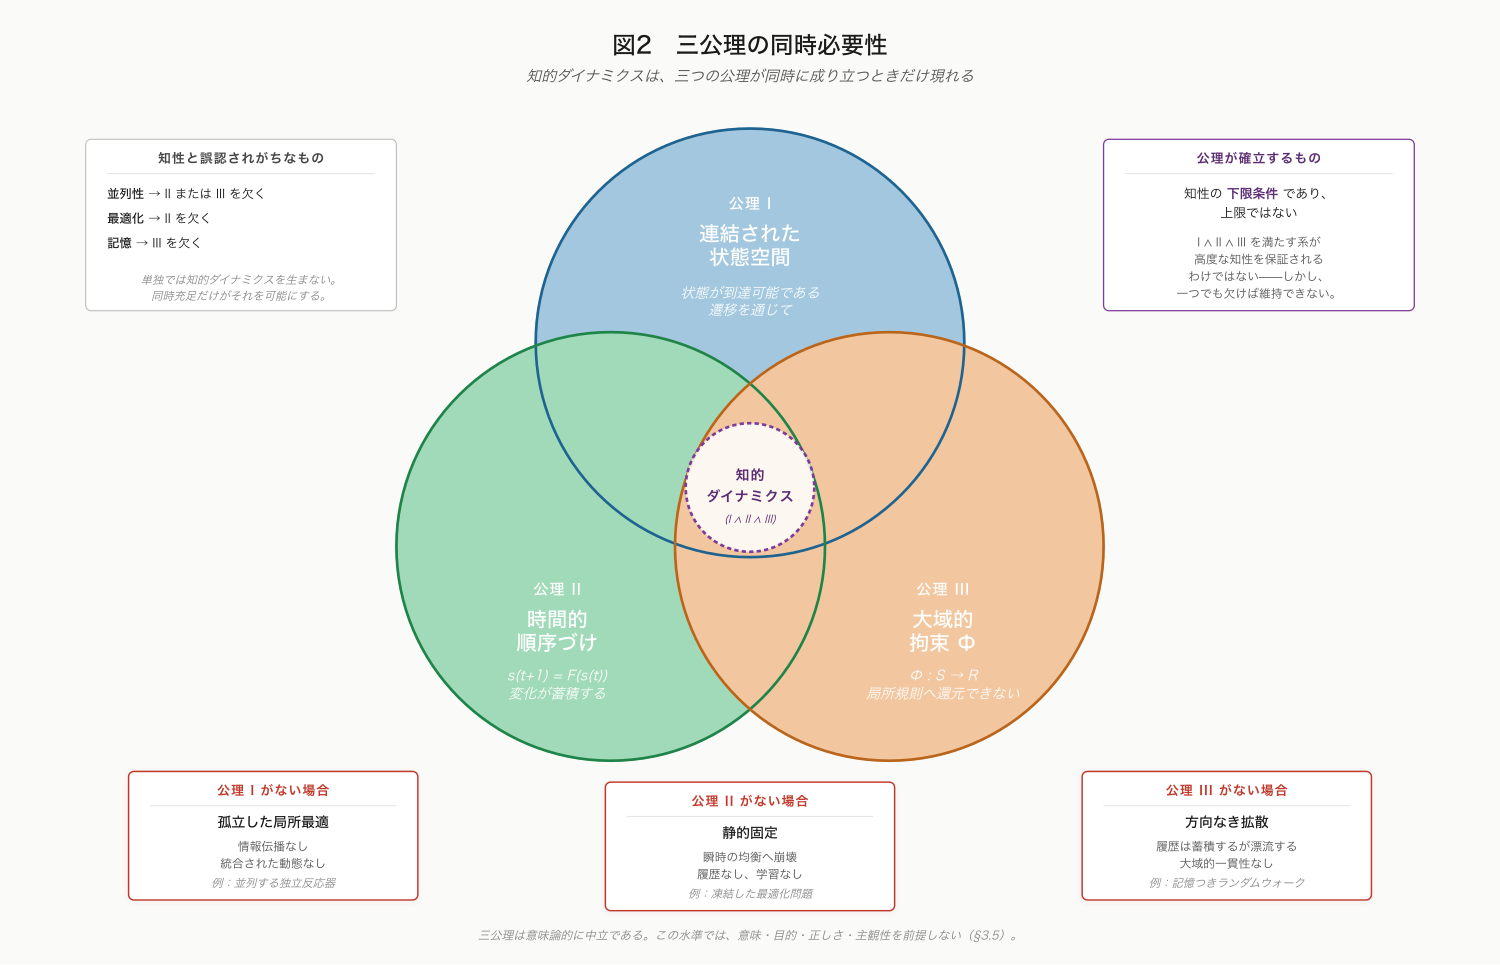
\includegraphics[width=\textwidth]{figures/fig2_three_axioms_ja.png}
\caption{三公理の同時必要性(三条件のベン図的配置と、各公理を欠いた場合の退化様式)}
\label{fig:intelligence_part1_2}
\end{figure}
